%% ============================================================
%%  Engineering Applications of Artificial Intelligence submission
%%  "Bitcoin Daily Direction Prediction via Dual-Encoder Cross-Attention:
%%   On-Chain Metrics, Walk-Forward Validation and Uncertainty-Aware Trading"
%%
%%  Template : Elsevier elsarticle, final 3p single-column (author-year)
%%  Compiled with: pdflatex + bibtex  (or Overleaf)
%% ============================================================

%%\documentclass[preprint,12pt,authoryear]{elsarticle}
%%\documentclass[authoryear,preprint,review,12pt]{elsarticle}
%% Use the options 1p,twocolumn; 3p; 3p,twocolumn; 5p; or 5p,twocolumn
%% for a journal layout:
%%\documentclass[final,1p,times,authoryear]{elsarticle}
%%\documentclass[final,1p,times,twocolumn,authoryear]{elsarticle}
 \documentclass[final,3p,times,authoryear]{elsarticle}
%%\documentclass[final,3p,times,twocolumn,authoryear]{elsarticle}
%%\documentclass[final,5p,times,authoryear]{elsarticle}
%%\documentclass[final,5p,times,twocolumn,authoryear]{elsarticle}

\usepackage{amssymb}
\usepackage{amsmath}
\usepackage{xcolor}
\usepackage{url}
\usepackage{booktabs}
\usepackage{multirow}
\usepackage{float}
\usepackage{array}
\usepackage{algorithm}
\usepackage{algpseudocode}
\usepackage{subcaption}
\usepackage{tikz}
\usetikzlibrary{shapes.geometric, arrows.meta, positioning, fit, backgrounds}

% -- Tikz arrow styles ---------------------------------------------------------
\tikzset{
  block/.style  = {rectangle, rounded corners=4pt, draw=black!70,
                   fill=blue!10, minimum width=2.8cm, minimum height=0.7cm,
                   align=center, font=\small},
  ablock/.style = {rectangle, rounded corners=4pt, draw=orange!80,
                   fill=orange!15, minimum width=2.8cm, minimum height=0.7cm,
                   align=center, font=\small},
  arrow/.style  = {-Stealth, thick},
  dasharrow/.style = {-Stealth, dashed, thick, gray}
}

\journal{Engineering Applications of Artificial Intelligence}

\begin{document}

\begin{frontmatter}

\title{Bitcoin Direction Prediction via Dual-Encoder Cross-Attention:
  Interpretability and Uncertainty-Aware Trading}

%% use optional labels to link authors explicitly to addresses:
\author[a]{Author One\corref{cor1}}
\ead{corresponding@university.edu}

\author[a,b]{Author Two}
\ead{author2@university.edu}

\cortext[cor1]{Corresponding author}

\address[a]{Department of Computer Science, University Name, City, Country}
\address[b]{Department of Finance, University Name, City, Country}

\begin{abstract}
This study investigates the performance of Machine Learning (ML) and Deep
Learning (DL) models in predicting the next-day direction of Bitcoin price
returns, with direct application to long/short algorithmic trading strategies.
The model inputs comprise Bitcoin on-chain blockchain metrics and classical
technical analysis indicators.
The ML and DL models evaluated include Support Vector Machines (SVM), XGBoost,
LightGBM, Convolutional Neural Network-Long Short-Term Memory (CNN-LSTM), and
a Multilayer Perceptron (MLP).
A central contribution of this study is the proposed Dual-Encoder
Cross-Attention (DECA) architecture, which routes each input type through
independent residual encoders and integrates their cross-domain interactions
via cross-attention, providing interpretable attention weights and
uncertainty-aware predictions through Monte Carlo Dropout.
An important methodological aspect is the adoption of an expanding-window
walk-forward cross-validation protocol covering six annual folds from 2019
to 2024, which offers more rigorous temporal validation than the simple
train-test splits commonly adopted in the literature.
The findings reveal that DECA achieves the highest Matthews Correlation
Coefficient (MCC = 0.648) among all models evaluated, while remaining
statistically equivalent to SVM in directional accuracy.
Static models generally outperformed sequence models under this evaluation
protocol.
It was found that on-chain blockchain metrics provide substantially greater
directional signal than technical indicators alone, corroborating and extending
recent findings in the literature.
Finally, the study assessed model profitability through backtesting by
replicating the conditions of prior work, and DECA emerged as the most
profitable deterministic model.
A dynamic confidence threshold on the Monte Carlo uncertainty further improved
returns.
This study emphasizes the importance of evaluation methodology, architecture
design, and input data type in Bitcoin price direction prediction.
The findings offer practitioners principled tools for uncertainty-aware trading
decisions and improved investment outcomes.
\end{abstract}

\begin{highlights}
\item Walk-forward cross-validation (CV) exposes optimistic bias in simple train-test splits, reversing CNN-LSTM (Convolutional Neural Network -- Long Short-Term Memory) performance.
\item The proposed DECA (Dual-Encoder Cross-Attention) architecture achieves the highest Matthews Correlation Coefficient (MCC\,=\,0.648) among all evaluated models.
\item On-chain blockchain metrics provide approximately ten times more predictive signal than technical indicators alone.
\item Monte Carlo (MC) Dropout raises prediction accuracy to 96.4\% at 50\% coverage via calibrated uncertainty filtering.
\item A dynamic MC confidence threshold achieves 4{,}013\%/year annualised return, surpassing deterministic DECA (3{,}922\%) in backtesting.
\end{highlights}

\begin{keyword}
Bitcoin \sep price direction prediction \sep walk-forward cross-validation \sep
dual-encoder architecture \sep cross-attention \sep on-chain metrics \sep
Monte Carlo Dropout \sep uncertainty quantification \sep backtesting \sep SHAP
\end{keyword}

\end{frontmatter}

%% ============================================================
\section{Introduction}
\label{sec:intro}
%% ============================================================

Bitcoin remains the world's largest cryptocurrency by market
capitalisation \citep{coinmarketcap2024}, with daily returns frequently
exceeding $\pm$5\% and structural regime changes driven by halving
cycles, institutional adoption, and regulatory developments
\citep{baur2018bitcoin, dyhrberg2016bitcoin}.
Predicting the \emph{direction} of next-day returns (binary
classification: up or down) is more directly actionable than
point-value regression, as it maps cleanly to long/short trading
decisions while remaining less sensitive to magnitude errors.

A substantial body of research has addressed this problem over the past
decade, achieving self-reported accuracies in the range of 75--83\%
\citep{mcnally2018predicting, omole2024financial, omole2025eaai}.
However, the majority of these results are obtained on a single 80/20
train-test split, a protocol known to produce optimistically biased
estimates when applied to time-series data
\citep{bergmeir2012time, tashman2000out}.
As we show in Section~\ref{sec:results}, results for sequence-based models
differ substantially across evaluation protocols, and the gap between
simple-split and walk-forward estimates can be considerable, consistent
with the time-series CV literature
\citep{bergmeir2012time, tashman2000out}.

A second limitation of prior work is the separation between technical
and on-chain features.
\citet{omole2024financial} used only on-chain metrics;
\citet{omole2025eaai} subsequently combined both sources
but processed them as a single flat feature vector.
Neither study exploited the structural complementarity between these two
domains through an architecture designed to model their interaction
explicitly: technical indicators summarise price dynamics, while on-chain
metrics encode blockchain-level investor behaviour.

In this paper we address both limitations with four contributions:

\begin{enumerate}

  \item Dual-Encoder Cross-Attention (DECA) architecture.
  We introduce DECA, a model that routes technical indicators and on-chain
  metrics through domain-specific deep MLP encoders, then learns
  cross-domain interactions via bidirectional cross-attention
  \citep{vaswani2017attention} with learnable context tokens and gated
  fusion.
  Under walk-forward CV, DECA achieves MCC\,=\,0.648, the highest
  across all five models evaluated.
  DECA and SVM (MCC\,=\,0.633) form a statistically equivalent top tier
  (McNemar $p=1.0$); their differentiation lies in operational
  capabilities: DECA's cross-attention weights provide domain-level
  interpretability and MC Dropout yields calibrated uncertainty estimates
  unavailable to kernel methods.

  \item Rigorous walk-forward evaluation with Bayesian hyperparameter
  optimisation.
  We apply a six-fold expanding-window cross-validation protocol
  covering 2019--2024, with Optuna TPE optimisation
  \citep{akiba2019optuna} running 50 trials per model independently on
  each architecture.
  Statistical significance is assessed via McNemar's test
  \citep{dietterich1998mcnemar} with Bonferroni correction over 10
  pairwise comparisons ($\alpha = 0.005$).
  This methodology directly addresses the evaluation gap identified in
  prior work \citep{bergmeir2012time}.

  \item MC Dropout uncertainty quantification for actionable trading.
  We apply Monte Carlo Dropout \citep{gal2016dropout} to DECA at no
  retraining cost (30 stochastic passes), obtaining well-calibrated
  epistemic uncertainty.
  Filtering to the 50\% most confident predictions raises accuracy to
  96.4\% (2019--2024), enabling principled coverage--accuracy trade-offs
  in practical trading strategies.

  \item Ablation study over four feature groups.
  We quantify the individual contribution of OHLCV, technical indicators,
  and on-chain metrics via XGBoost ablation.
  On-chain metrics alone (G2) outperform technical indicators alone (G1)
  by a factor of approximately ten in MCC (0.387 vs.\ 0.036),
  corroborating and extending the findings of \citet{omole2025eaai}.

\end{enumerate}

The remainder of the paper is organized as follows.
Section~\ref{sec:related} reviews related work.
Section~\ref{sec:data} describes the dataset and feature engineering.
Section~\ref{sec:method} details the proposed architecture, baselines,
and evaluation protocol.
Section~\ref{sec:results} presents quantitative results and analysis.
Section~\ref{sec:conclusion} concludes.

%% ============================================================
\section{Related Work}
\label{sec:related}
%% ============================================================

\subsection{Bitcoin Direction Prediction}

Early machine learning approaches to Bitcoin price prediction followed
stock-market paradigms, applying SVMs, random forests, and LSTMs to
price-derived technical indicators \citep{mcnally2018predicting,
patel2015predicting}.
A common finding is that no single architecture consistently dominates
across evaluation windows \citep{ji2019bitcoin}, and that results are
heavily dependent on the choice of train-test split.

Subsequent work incorporated alternative data sources, most notably
social media sentiment.
\citet{zhang2021sentiment} demonstrated that Twitter sentiment polarity
provides a statistically significant leading signal for next-day Bitcoin
returns, and \citet{abraham2018crypto} showed that Reddit discussion
volume correlates with short-term volatility spikes.
Hybrid models that concatenate sentiment embeddings with price-derived
features have been shown to improve directional accuracy over price-only
baselines \citep{li2020hybrid}, though the gains tend to degrade
during periods of abnormally high posting volume such as market crashes.

Several studies have designed architectures specifically for
cryptocurrency rather than adapting stock-market models.
\citet{lahmiri2019cryptocurrency} showed that LSTM networks trained on
hourly crypto data exhibit markedly different loss landscapes than
equivalent models on equity indices, attributing this to the fat-tailed
return distribution and the absence of circuit breakers in 24/7 markets.
The problem of non-stationarity is particularly acute: Bitcoin has
transitioned through at least three structurally distinct regimes
(retail speculation before 2017, institutional entry in 2020--2022, and
spot-ETF-driven adoption from 2024 onward), and a model calibrated in
one regime may be effectively out-of-distribution in the next
\citep{bouri2019regime}.
Empirical evidence from this and related studies suggests that model
performance can collapse abruptly when the underlying market structure
shifts, consistent with a structural break rather than a recoverable
noise floor.

\citet{omole2024financial} conducted a comprehensive study
using 87 on-chain features and deep learning models (CNN-LSTM, LSTNet,
TCN) with Boruta feature selection.
With a CNN-LSTM on Boruta-selected features, they reported
Accuracy\,=\,82.4\%, MCC\,=\,0.649, AUC\,=\,0.824 on a single 80/20
split of weekly Bitcoin data and demonstrated profitable backtesting
results (6{,}653\%/year annualised return).

\citet{omole2025eaai} subsequently combined
on-chain data with technical indicators (225 features total, Boruta
selection) and found that SVM achieved the best accuracy (83\%) on a
simple holdout, while deep learning models (CNN-LSTM, TCN) performed
comparably or worse.
Crucially, technical indicators alone yielded only 50--53\% accuracy
(near-random), corroborating the finding replicated by our G1
ablation.
Our work extends both studies by (a) evaluating under walk-forward CV
rather than simple splits, (b) introducing an architecture that
explicitly models the interaction between technical and on-chain domains,
and (c) providing uncertainty quantification applicable to risk-controlled
trading strategies.

\subsection{On-Chain Metrics as Predictive Signals}

Blockchain transactions produce a publicly auditable trail of economic
activity that has no direct analogue in traditional asset markets.
Unlike equities, where fundamental data is disclosed quarterly and
subject to accounting discretion, Bitcoin's ledger is continuously
observable at transaction granularity.

Derived metrics synthesise this raw activity into economically
interpretable signals.
MVRV (Market Value to Realised Value) compares market capitalisation with
the aggregate cost basis of all circulating coins; values below 1.0
historically correspond to accumulation phases that have preceded major
bull markets \citep{glassnode2020mvrv}.
SOPR (Spent Output Profit Ratio) measures the ratio of the USD value of
coins at time of spending to their value at acquisition; sustained values
below 1.0 signal that holders are capitulating at a loss \citep{kent2018sopr}.
Short-Term Holder SOPR (STH-SOPR) isolates coins moved within the past
155 days and functions as a real-time market stress indicator: sharp drops
below 1.0 often mark local price floors.
NVT (Network Value to Transactions) is a valuation ratio analogous to
price-to-earnings; high NVT values suggest market capitalisation is running
ahead of on-chain economic throughput, historically preceding corrections
\citep{liv2019nvt}.
The consistent finding across multiple independent studies that on-chain
metrics substantially outperform technical indicators in isolation
\citep{omole2024financial, omole2025eaai} motivates their inclusion as
the primary predictive domain, and our G1 vs.\ G2 ablation provides
additional empirical evidence under walk-forward CV conditions that are
less susceptible to overfitting artefacts.

\subsection{Attention Mechanisms and Dual-Encoder Architectures in Finance}

The Transformer architecture \citep{vaswani2017attention} replaced
recurrence with scaled dot-product self-attention, enabling
parallelisable modelling with direct long-range dependencies.
Financial applications quickly followed: \citet{wu2021autoformer}
introduced decomposition-based attention for long-horizon time-series
forecasting, and attention-based models have been applied to
event-driven stock prediction \citep{ding2020transformer}.

Cross-attention, in which queries from one sequence attend to keys and
values from a second, distinct sequence, is the natural mechanism
for fusing heterogeneous data streams.
Dual-encoder architectures encode two input domains independently before
combining their representations; this design preserves domain-specific
inductive biases while allowing a fusion layer to learn cross-domain
interactions.
For tabular financial data, self-attention applied within a single
feature vector treats all features symmetrically, which is suboptimal
when features originate from two structurally distinct generating
processes (price mechanics vs.\ blockchain economics).
Our architecture addresses this by routing technical indicators and
on-chain metrics through separate MLP branches before stacking
bidirectional cross-attention layers, ensuring each domain can act as a
conditioning context for the other.
To our knowledge, this is the first application of a dual-encoder
cross-attention architecture to the fusion of on-chain and technical
feature domains for cryptocurrency direction prediction.

\subsection{Uncertainty Quantification in Algorithmic Trading}

Standard point-estimate classifiers assign a label without conveying
confidence, which is problematic in finance where the costs of false
positives and false negatives are asymmetric and time-varying.
MC Dropout \citep{gal2016dropout} interprets dropout at inference time
as approximate variational inference, enabling Monte Carlo estimation of
predictive variance at negligible computational cost.
Deep Ensembles \citep{lakshminarayanan2017simple} aggregate predictions
from multiple independently initialised networks and have been shown to
produce well-calibrated uncertainty, particularly in out-of-distribution
regimes.

In algorithmic trading, uncertainty estimates enable selective
prediction \citep{geifman2017selective}: the model abstains on
low-confidence days and trades only when uncertainty falls below a
threshold.
This coverage-accuracy tradeoff is directly exploitable as a risk
management tool, and the asymmetric loss structure of trading (a missed
opportunity costs less than a wrong directional bet at peak leverage)
motivates treating uncertainty as a first-class output rather than a
diagnostic afterthought.

\subsection{Evaluation Methodology}

A recurring concern in financial machine learning is methodological
overfitting: hyperparameters and architectures are tuned on the same
period used for evaluation, producing optimistically biased results
\citep{tashman2000out, arlot2010survey}.
Walk-forward or rolling-origin cross-validation has been advocated as a
principled remedy \citep{bergmeir2012time}, yet most cryptocurrency
prediction papers continue to use simple splits.

The problem is compounded by implicit multiple comparisons: when many
model variants are screened against the same holdout, the probability
that at least one exceeds a performance threshold by chance grows
rapidly \citep{harvey2016p}.
Bonferroni correction provides conservative family-wise error rate
control; we apply it to all McNemar and Wilcoxon pairwise tests.
Cryptocurrency data poses additional challenges: the absence of
closing auctions, 24/7 trading, and episodic structural breaks
violate stationarity assumptions underlying classical CV theory.
\citet{lopezdeprado2018advances} proposes combinatorial purged
cross-validation with embargo periods to prevent leakage through
overlapping labels; our expanding-window design achieves the same
leakage prevention by construction, since each test fold is strictly
future to all training data.

The 82.4\% accuracy reported by \citet{omole2024financial} was obtained
under a single 80/20 split with a different feature set and experimental
conditions; under our walk-forward protocol the same architecture achieves
MCC\,$\approx$\,0.01 with default hyperparameters and MCC\,=\,0.453 after
full Optuna tuning.
Whether the discrepancy is attributable to the evaluation protocol, the
feature selection procedure, or other implementation details cannot be
determined without access to the original code, and we make no claim
beyond reporting what we observe under our own experimental setup.
We argue that MCC \citep{chicco2020mcc} should be the primary evaluation
metric, as it is invariant to class imbalance and provides a balanced
measure of discriminative power.

%% ============================================================
\section{Data and Feature Engineering}
\label{sec:data}
%% ============================================================

\subsection{Dataset}

We construct a daily dataset spanning January 2013 to December 2024 by
merging two data sources:
(i) OHLCV (Open, High, Low, Close, Volume) price data from
CoinGecko/Binance, and (ii) on-chain metrics from Glassnode, comprising
33 features in total.
After forward-filling and backward-filling residual missing values (which
arise from weekend data gaps in some on-chain series prior to 2016), the
dataset contains 4{,}383 daily observations.
The binary target variable $y_t \in \{0,1\}$ is defined as
$y_t = \mathbf{1}[\text{Close}_{t+1} > \text{Close}_t]$, i.e., whether
the closing price the \emph{next} day is higher than the current day.
The positive class (price up) comprises approximately 54.1\% of all days,
indicating a mild positive drift consistent with the literature.

\subsection{Feature Groups}

We define four feature groups to support our ablation study
(Table~\ref{tab:feature_groups}):

\begin{table}[ht]
\centering
\caption{Feature group definitions used in the ablation study.
  $|\cdot|$ denotes the number of features in each group.}
\label{tab:feature_groups}
\small
\begin{tabular}{lll p{6cm}}
\hline
Group & $|F|$ & Label & Description \\
\hline
G0 & 5  & OHLCV       & Raw market data only (baseline) \\
G1 & 15 & OHLCV+Tech  & G0 + 10 technical indicators \\
G2 & 23 & OHLCV+Chain & G0 + 18 on-chain metrics \\
G3 & 33 & Full        & G0 + Technical + On-Chain (union of G1 and G2) \\
\hline
\end{tabular}
\end{table}

\noindent Technical indicators (10 features, routed to the
\emph{technical branch} of DECA):
RSI-14, Stochastic-K\textsubscript{14,3}, Stochastic-D\textsubscript{14,3},
Bollinger \%B\textsubscript{20}, OBV (on-balance volume),
distance-to-SMA200, 30-day ROI, drawdown from all-time high,
30-day Sharpe ratio, and 1-day log-return.
These indicators are computed over the entire history and then split per
fold, so no future information leaks into earlier folds.

\noindent On-chain metrics (18 features, routed to the
\emph{on-chain branch} of DECA):
MVRV ratio, Realised Price, Short-Term Holder SOPR,
Supply in Loss (absolute and percentage), SOPR (day-1 lag),
Net Realised Profit and Loss (NRPL), UTXOs in Loss (absolute and
percentage), Adjusted SOPR (aSOPR), Price-to-Realised ratio,
MVRV Z-score (365-day), Supply in Profit (percentage and absolute),
UTXOs in Profit (percentage), Market Cap--MVRV product (CapMVRVCur),
Net Unrealised Loss (NUL), and Realised Cap UTXO Age Bands percentage.

\subsection{Feature Selection Rationale}
\label{sec:feature_rationale}

The 33 features comprising G3 were selected following three complementary
criteria.

\noindent (1) Empirical evidence from prior literature.
\citet{omole2024financial} applied Boruta feature selection over 87
on-chain metrics and consistently identified the SOPR and MVRV families
as the most predictive signals for daily Bitcoin direction.
\citet{omole2025eaai} confirmed that on-chain metrics substantially
outperform technical indicators used in isolation, a finding
replicated by our G1 vs.\ G2 ablation (Section~\ref{sec:ablation}).

\noindent (2) Systematic coverage of distinct market dimensions.
The feature set captures complementary aspects of market behaviour:
the 5 OHLCV variables provide raw price dynamics;
the 10 technical indicators span \emph{momentum} (RSI-14, Stochastic K/D,
30-day ROI, 1-day log-return), \emph{trend} (distance to SMA-200,
drawdown from ATH), \emph{volatility} (Bollinger \%B, 30-day Sharpe
ratio) and \emph{volume flow} (OBV);
and the 18 on-chain metrics cover \emph{holder profitability}
(SOPR, aSOPR, NRPL, Supply/UTXOs in Profit and Loss)
and \emph{market valuation relative to realised value}
(MVRV, MVRV Z-score, Price-to-Realised, CapMVRVCur).

\noindent (3) Public availability without survivorship bias.
All features are sourced from Glassnode and standard OHLCV providers,
available for the entire study period (2013--2024).
Their predictive relevance is confirmed a posteriori by SHAP analysis
(Section~\ref{sec:shap}): Short-Term Holder SOPR ranks first across all
folds, and 5 of the top-10 SHAP features belong to the on-chain group.

\begin{figure}[h!]
  \centering
  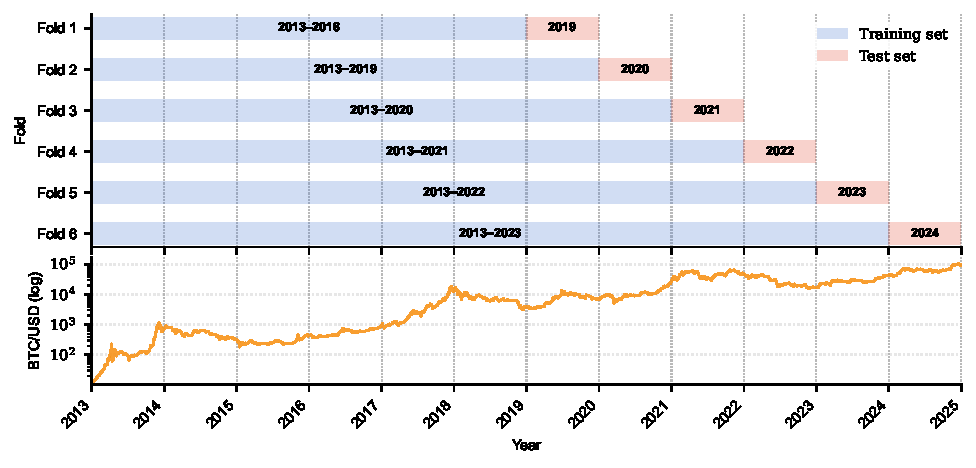
\includegraphics[width=\linewidth]{figures/fig1_walk_forward_diagram.pdf}
  \caption{Walk-forward expanding-window cross-validation protocol
    (six folds, 2019--2024 test windows).
    Each fold uses all available history up to the test year as training
    data. The bottom panel shows the Bitcoin closing price (log scale)
    over the study period for reference.}
  \label{fig:wfcv}
\end{figure}

\subsection{Walk-Forward Cross-Validation}
\label{sec:wfcv}

We apply an expanding-window walk-forward protocol with six folds,
each using one calendar year as the test set (2019--2024), as
illustrated in Figure~\ref{fig:wfcv}.
The training set for fold $k$ includes all data from the start of the
dataset up to the end of year $2018+k-1$.
This design eliminates look-ahead bias and mimics realistic deployment
conditions.
Feature scaling (RobustScaler \citep{muller1997robust}) and
class-imbalance weights are fitted exclusively on the training portion
of each fold.

%% ============================================================
\section{Methodology}
\label{sec:method}
%% ============================================================

\subsection{Dual-Encoder Cross-Attention (DECA) Architecture}
\label{sec:deca}

A central design question in multi-source financial prediction is
\emph{how} to combine heterogeneous feature streams without destroying
the structure inherent to each.
A straightforward approach is to concatenate all features into a single
vector and process them through a unified network, treating every input
dimension symmetrically.
This is a natural starting point and is precisely the configuration we
evaluate as the MLP-Simple baseline (Section~\ref{sec:arch_ablation}).
However, when the input features originate from two structurally
distinct generating processes (price-derived momentum signals on one
side and blockchain-level economic indicators on the other), a single
shared transformation must simultaneously model intra-domain
relationships within each group \emph{and} inter-domain interactions
between them.
Prior work on multi-source representation learning has argued that this
conflation can hinder the learning of domain-specific structure
\citep{ngiam2011multimodal}, and our ablation results provide direct
empirical evidence in this setting: MLP-Simple achieves MCC\,=\,0.450,
while routing the same features through independent domain encoders
without cross-attention (MLP-DualNoAttn) raises MCC to 0.556
($+$0.106), as discussed in detail in
Section~\ref{sec:arch_ablation}.

The design philosophy of DECA is to \emph{separate before fusing}.
Each feature domain is first processed independently by a dedicated
deep encoder whose architecture is optimised for the statistical
structure of that domain.
Only after both domains have been compressed into compact, informative
representations does the model attempt to learn cross-domain
interactions, doing so through a principled attention
mechanism that can dynamically weight the relevance of one domain's
representation to the other, conditioned on the specific input at hand.
The result is a form of contextual cross-domain reasoning that is
structurally impossible in flat feature-concatenation models, enabling
the model to answer questions of the form
\emph{"given the current on-chain stress signals, how much should the
technical momentum context reinforce or dampen the directional forecast?"}

Concretely, DECA is organized into four functional stages, each of
which is described below and illustrated in Figure~\ref{fig:deca}:
(i) independent domain encoding via deep residual MLPs,
(ii) context token augmentation,
(iii) bidirectional cross-attention, and
(iv) gated fusion followed by binary classification.

\begin{figure}[h!]
  \centering
  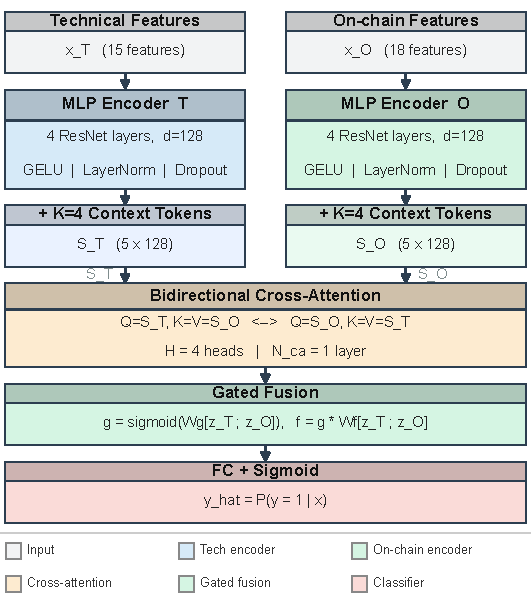
\includegraphics[width=90mm]{figures/fig_deca_architecture.pdf}
  \caption{DECA architecture overview.
    Technical and on-chain features are encoded by independent MLP
    branches ($L=4$ residual layers, $d=128$).
    Each encoder output is augmented with $K=4$ learnable context tokens
    and passed through a bidirectional cross-attention block.
    The resulting representations are merged by a gated fusion layer
    before binary classification.}
  \label{fig:deca}
\end{figure}

\noindent Stage 1: Domain-Specific MLP Encoder.
Each branch receives its domain's input vector
$\mathbf{x} \in \mathbb{R}^d$ (where $d=15$ for the technical branch
and $d=18$ for the on-chain branch) and projects it into a shared
latent space of dimension $d_h$ through a linear embedding layer
$\mathbf{h}^{(0)} = W_0\,\mathbf{x}$.
The embedding is then refined by $L=4$ stacked residual blocks of the form:
\begin{equation}
  \mathbf{h}^{(\ell)} = \mathrm{LayerNorm}\!\left(
    \mathbf{h}^{(\ell-1)} + \mathrm{GELU}\!\left(
      W_2^{(\ell)}\,\mathrm{GELU}\!\left(W_1^{(\ell)}\mathbf{h}^{(\ell-1)}\right)
    \right)
  \right),
\end{equation}
where $d_h=128$ and all weight matrices $W_i^{(\ell)} \in
\mathbb{R}^{d_h \times d_h}$.
The residual connection prevents gradient vanishing in deep stacks
\citep{he2016deep}, while Layer Normalisation \citep{ba2016layer}
stabilises training across folds with heterogeneous feature distributions.
Dropout \citep{srivastava2014dropout} with rate $p=0.333$ is applied
after each non-linearity to act as both a regulariser and, at inference
time, as the stochastic mechanism for MC Dropout uncertainty estimation
(Section~\ref{sec:mc_dropout}).
The output of the encoder, $\mathbf{z} = \mathbf{h}^{(L)} \in
\mathbb{R}^{d_h}$, is a compact, intra-domain summary that has
learned feature interactions (e.g., co-movement of STH-SOPR and
MVRV) without any awareness of the other domain.

\noindent Stage 2: Context Token Augmentation.
A single vector $\mathbf{z}$ provides no natural sequence structure
over which attention can operate.
Following the prompt-tuning paradigm of \citet{lu2021pretrained},
we augment each encoder output with $K=4$ learnable context tokens
$\{\mathbf{c}_k\}_{k=1}^K \in \mathbb{R}^{d_h}$, forming an
augmented sequence $\mathbf{S} = [\mathbf{z},\, \mathbf{c}_1,
\ldots, \mathbf{c}_K] \in \mathbb{R}^{(K+1) \times d_h}$.
The context tokens serve as soft, trainable query anchors that allow
the cross-attention mechanism to attend selectively to different
aspects of the opposing domain's representation.
Intuitively, one context token may learn to query for
\emph{"is the on-chain cost basis above market price?"}
while another queries \emph{"is momentum aligned with on-chain
selling pressure?''} Such specialisations emerge purely from
gradient optimisation.

\noindent Stage 3: Bidirectional Cross-Attention.
Let $\mathbf{S}_T$ and $\mathbf{S}_O$ denote the augmented sequences
for the technical and on-chain branches respectively.
Cross-attention is applied symmetrically in both directions using
$H=4$ attention heads \citep{vaswani2017attention}:
\begin{align}
  \mathbf{S}_T' &= \mathrm{CrossAttn}(Q\!=\!\mathbf{S}_T,\;
                                      K\!=\!\mathbf{S}_O,\;
                                      V\!=\!\mathbf{S}_O),\\
  \mathbf{S}_O' &= \mathrm{CrossAttn}(Q\!=\!\mathbf{S}_O,\;
                                      K\!=\!\mathbf{S}_T,\;
                                      V\!=\!\mathbf{S}_T).
\end{align}
The first operation asks: \emph{"given the technical representation,
which aspects of the on-chain context are most informative?"}
The second asks the symmetric question.
Because the interaction is bidirectional, neither domain is treated as
a subordinate conditioning signal; both domains simultaneously enrich
each other's representation, which is critical for capturing
asymmetric information flows (confirmed empirically in
Section~\ref{sec:attention}: on-chain representations benefit more
from technical context than vice versa).

\noindent Stage 4: Gated Fusion and Classification.
The updated first tokens $\hat{\mathbf{z}}_T$ and $\hat{\mathbf{z}}_O$
(the positions corresponding to the original encoder outputs in
$\mathbf{S}_T'$ and $\mathbf{S}_O'$) are concatenated and passed
through a gated fusion layer:
\begin{equation}
  \mathbf{g} = \sigma\!\left(W_g[\hat{\mathbf{z}}_T;\hat{\mathbf{z}}_O]\right),
  \qquad
  \mathbf{f} = \mathbf{g} \odot W_f[\hat{\mathbf{z}}_T;\hat{\mathbf{z}}_O].
\end{equation}
The sigmoid gate $\mathbf{g}$ learns to weight the contribution of
each domain to the final representation $\mathbf{f}$, providing an
additional degree of adaptability beyond the attention weights.
A final linear layer maps $\mathbf{f}$ to a scalar logit; the
predicted probability of an upward move is $\hat{p} = \sigma(\mathbf{f})$.

\subsection{Baseline Models}

Four external baselines are evaluated under the same walk-forward
protocol and Optuna hyperparameter search (50 trials, TPE sampler)
as DECA, ensuring a fair comparison in which no model benefits from
a more favourable evaluation procedure.
The selection covers three distinct model families: gradient-boosted
trees, kernel methods, and sequence neural networks.
SVM and CNN-LSTM are included as state-of-the-art references, as they
represent the best-performing models reported by \citet{omole2025eaai}
and \citet{omole2024financial}, respectively.

\begin{description}

  \item[XGBoost-G3] \citep{chen2016xgboost}
    Extreme Gradient Boosting trains an ensemble of decision trees
    sequentially, with each tree correcting the residuals of the
    previous one using second-order gradient information.
    XGBoost is widely considered the most competitive non-neural
    baseline for tabular data \citep{grinsztajn2022tree} and
    provides a strong reference point for assessing whether a
    neural architecture offers any benefit beyond powerful
    feature interactions learnable from trees.
    It operates on the full 33-feature vector (G3) without any
    domain separation.

  \item[LightGBM-G3] \citep{ke2017lightgbm}
    LightGBM is a gradient-boosted tree framework that grows trees
    leaf-wise (best-first) rather than level-wise, which tends to
    reduce loss more aggressively per iteration at the cost of
    higher variance on small datasets.
    On large tabular datasets it often matches or slightly outperforms
    XGBoost in accuracy while being significantly faster to train.
    Its inclusion alongside XGBoost allows us to assess whether the
    tree-ensemble tier result is robust to the choice of boosting
    implementation.

  \item[SVM-G3] \citep{cortes1995svm}
    Support Vector Machines with an RBF kernel find the maximum-margin
    hyperplane in a kernel-induced feature space, making them
    effective in high-dimensional settings where decision boundaries
    are non-linear.
    SVM was the strongest model reported by \citet{omole2025eaai}
    (83\% accuracy on a simple holdout), making it the most directly
    comparable external baseline.
    Input features are standardised per fold with a StandardScaler
    applied after the global RobustScaler, as SVMs are sensitive to
    feature scale.

  \item[CNN-LSTM-G3] \citep{lecun2015deep}
    The CNN-LSTM architecture combines a one-dimensional convolutional
    layer, which extracts local temporal patterns over a sliding
    window of $T$ days, with a stacked LSTM that models longer-range
    sequential dependencies in the resulting feature maps.
    This architecture directly replicates the design of
    \citet{omole2024financial}, who reported 82.4\% accuracy on a
    simple split and attributed the result to the model's ability to
    learn multi-scale temporal structure from on-chain data.

\end{description}

\noindent Three additional DECA architecture ablation variants
(MLP-Simple, MLP-DualNoAttn, DECA-FE) are defined and evaluated
separately in Section~\ref{sec:arch_ablation} to isolate the
contribution of each architectural component.

\subsection{Hyperparameter Optimisation}
\label{sec:hyper}

All models are tuned with Optuna \citep{akiba2019optuna} using the
Tree-structured Parzen Estimator (TPE) sampler \citep{bergstra2011tpe},
which builds probabilistic surrogate models of the objective function
and exploits regions of high expected improvement, generally requiring
far fewer trials than grid or random search to reach near-optimal
configurations.
We run 50 trials per model with a Median Pruner (10 warm-up trials) to
discard unpromising configurations early, a fixed random seed for
reproducibility, and the mean MCC across all six folds as the
optimisation objective.
Using the full cross-validation mean as the objective rather than a
single validation fold is critical: it prevents Optuna from selecting
hyperparameters that are optimal for one particular market regime
but fail to generalise across the 2019--2024 period.

Table~\ref{tab:hyperspaces} reports the search space for DECA.
Each tree-based model (XGBoost, LightGBM) is searched over tree count,
depth, learning rate, subsampling ratios, and regularisation
coefficients; SVM over the kernel type, regularisation $C$, and kernel
width $\gamma$; CNN-LSTM over the sequence window, convolutional filter
count, LSTM hidden size, dropout, and learning rate.

\begin{table}[ht]
\centering
\caption{Hyperparameter search space for DECA (Optuna TPE, 50 trials).}
\label{tab:hyperspaces}
\small
\begin{tabular}{lll}
\hline
Hyperparameter & Range & Type \\
\hline
$d_h$ (hidden dim)           & $\{64, 128, 256, 512\}$  & categorical \\
Warmup epochs                & $[5, 20]$                 & integer \\
$H$ (attention heads)        & $\{2, 4, 8\}$             & categorical \\
$L$ (encoder layers)         & $[2, 6]$                  & integer \\
$N_{ca}$ (cross-attn layers) & $[1, 3]$                  & integer \\
Dropout rate                 & $[0.1, 0.5]$              & float \\
Learning rate                & $[10^{-4}, 10^{-2}]$      & log-float \\
Weight decay                 & $[10^{-5}, 10^{-1}]$      & log-float \\
Batch size                   & $\{16, 32, 64\}$          & categorical \\
Label smoothing $\varepsilon$& $[0, 0.2]$                & float \\
\hline
\end{tabular}
\end{table}

Table~\ref{tab:bestparams} reports the best configuration found for
each model, corresponding to the hyperparameters used in all results
reported in Section~\ref{sec:results}.

\begin{table}[H]
\centering
\caption{Best hyperparameter configuration selected by Optuna for each
  model (50 trials, TPE sampler). Values correspond to the setting that
  maximised mean MCC across folds 1--6.}
\label{tab:bestparams}
\small
\begin{minipage}[t]{0.47\linewidth}
\begin{tabular}{llr}
\hline
Model & Hyperparameter & Value \\
\hline
\multirow{9}{*}{XGBoost}
  & Trees                   & 900   \\
  & Max depth               & 3     \\
  & Learning rate           & 0.031 \\
  & Subsample               & 0.652 \\
  & Column subsample        & 0.504 \\
  & Min child weight        & 4     \\
  & Gamma                   & 2.251 \\
  & L1 regularisation       & 0.064 \\
  & L2 regularisation       & 0.051 \\
\hline
\multirow{9}{*}{LightGBM}
  & Trees                   & 1100      \\
  & Max depth               & 11        \\
  & Learning rate           & 0.036     \\
  & Subsample               & 0.560     \\
  & Column subsample        & 0.664     \\
  & Min child samples       & 93        \\
  & Num leaves              & 282       \\
  & L1 regularisation       & 2.57e{-6} \\
  & L2 regularisation       & 7.235     \\
\hline
\end{tabular}
\end{minipage}%
\hfill
\begin{minipage}[t]{0.47\linewidth}
\begin{tabular}{llr}
\hline
Model & Hyperparameter & Value \\
\hline
\multirow{5}{*}{SVM}
  & Kernel                  & poly      \\
  & $C$                     & 432.6     \\
  & $\gamma$                & 1.57e{-4} \\
  & Degree                  & 3         \\
  & Coef0                   & 4.573     \\
\hline
\multirow{8}{*}{CNN-LSTM}
  & Sequence window         & 5         \\
  & Conv filters            & 128       \\
  & LSTM hidden size        & 256       \\
  & LSTM layers             & 1         \\
  & Dropout rate            & 0.487     \\
  & Learning rate           & 1.43e{-3} \\
  & Weight decay            & 7.78e{-5} \\
  & Batch size              & 32        \\
\hline
\multirow{10}{*}{DECA}
  & Embedding dim $d_h$     & 64        \\
  & Attention heads $H$     & 4         \\
  & Encoder layers $L$      & 2         \\
  & Cross-attn layers $N_{ca}$ & 1      \\
  & Dropout rate            & 0.499     \\
  & Learning rate           & 4.74e{-4} \\
  & Weight decay            & 5.09e{-6} \\
  & Batch size              & 64        \\
  & Warmup epochs           & 14        \\
  & Label smoothing $\varepsilon$ & 0.068 \\
\hline
\end{tabular}
\end{minipage}
\end{table}

\noindent DECA training procedure.
The model is trained end-to-end with binary cross-entropy loss
\citep{muller2019labelsmoothing} and the AdamW optimiser
\citep{loshchilov2017adamw} with a linear warm-up over the first 5\%
of training steps followed by cosine decay.
Label smoothing ($\varepsilon = 0.068$, see Table~\ref{tab:bestparams})
reduces overconfidence on ambiguous days near the decision boundary, and
class-imbalance weights (positive-class weight $\approx 0.93$ given
54.1\% up-days) prevent the model from learning the majority-class prior.
The final values for all architectural and optimisation hyperparameters
are reported in Table~\ref{tab:bestparams}.

\subsection{Evaluation Metrics and Statistical Tests}

We adopt the Matthews Correlation Coefficient (MCC)
\citep{chicco2020mcc} as the primary evaluation criterion:
\begin{equation}
  \mathrm{MCC} = \frac{TP \cdot TN - FP \cdot FN}
    {\sqrt{(TP+FP)(TP+FN)(TN+FP)(TN+FN)}},
\end{equation}
where $TP$, $TN$, $FP$, and $FN$ denote true positives, true
negatives, false positives, and false negatives, respectively.
MCC is bounded in $[-1, 1]$, where $+1$ indicates perfect prediction,
$0$ is equivalent to random guessing, and $-1$ corresponds to total
disagreement with the true labels.
We prefer MCC over accuracy for three reasons.
First, it accounts for all four cells of the confusion matrix
simultaneously, whereas accuracy ignores the balance between false
positives and false negatives.
Second, MCC is provably invariant to class imbalance: a classifier
that always predicts the majority class scores $\mathrm{MCC} = 0$
regardless of the imbalance ratio, whereas its accuracy would
spuriously equal the majority-class frequency (54.1\% in our dataset).
Third, \citet{chicco2020mcc} demonstrate empirically that MCC is
the most informative single-number summary of binary classifier
performance, particularly for datasets with moderate imbalance such
as ours.

To facilitate comparison with prior work, we additionally report three
complementary metrics:
\begin{itemize}
  \item Accuracy ($\frac{TP+TN}{TP+TN+FP+FN}$): the fraction
    of correctly classified days. Widely reported in the literature but
    sensitive to class imbalance; included for comparability with
    \citet{omole2024financial, omole2025eaai}.
  \item AUC (Area Under the ROC Curve): measures
    discriminative ability across all classification thresholds,
    independent of the decision boundary. AUC $= 0.5$ corresponds to
    random ranking; AUC $= 1.0$ to perfect separation.
  \item Log-loss ($-\frac{1}{N}\sum_{i}[y_i \log \hat{p}_i +
    (1-y_i)\log(1-\hat{p}_i)]$): penalises overconfident wrong
    predictions and reflects the quality of the probability estimates
    rather than just the hard classification decision.
\end{itemize}

To assess whether differences between models are statistically
significant, we apply McNemar's test \citep{dietterich1998mcnemar} on the
concatenated binary predictions over the full evaluation set
(2{,}546 samples across folds 1--6).
McNemar's test is appropriate here because it directly evaluates
whether two classifiers disagree on the \emph{same} observations,
controlling for the correlation induced by using the same test samples.
We apply Bonferroni correction for 10 pairwise comparisons
($\alpha = 0.05 / 10 = 0.005$) to control the family-wise error rate.
We additionally report the Wilcoxon signed-rank test
\citep{wilcoxon1945individual} on per-fold MCC vectors as a secondary
fold-level consistency measure, which assesses whether performance
differences are systematic across folds rather than driven by a single
year.

\subsection{Computational Environment}
\label{sec:environment}

All experiments were conducted on a workstation running Windows~10 equipped
with an AMD Ryzen~5 3400G processor, 32\,GB of RAM, and an NVIDIA GeForce
RTX~5060~Ti GPU (16\,GB VRAM).
Neural network training used CUDA~12.8 via PyTorch~2.11
\citep{paszke2019pytorch}.
Additional libraries include scikit-learn~1.8 \citep{sklearn_api} for SVM
and preprocessing pipelines, XGBoost~3.2 \citep{chen2016xgboost},
LightGBM~4.6 \citep{ke2017lightgbm}, Optuna~4.8
\citep{akiba2019optuna} for Bayesian hyperparameter optimisation, and
SHAP~0.51 \citep{lundberg2017shap} for feature importance analysis.
All experiments are reproducible; source code and model artefacts are
publicly available at \url{https://github.com/HernanDiaz/BitcoinPricePrediction}.

%% ============================================================
\section{Results and Discussion}
\label{sec:results}
%% ============================================================

\subsection{Ablation Study: Feature Group Importance}
\label{sec:ablation}

Table~\ref{tab:ablation} reports XGBoost performance by feature group
(default hyperparameters, folds 1--6).

\begin{table}[ht]
\centering
\caption{Ablation study: XGBoost performance by feature group
  (folds 1--6, default hyperparameters). MCC values are mean $\pm$ std.}
\label{tab:ablation}
\small
\begin{tabular}{llccc}
\hline
Group & Description & Acc & MCC & AUC \\
\hline
G0 & OHLCV only        & $0.559\pm0.034$ & $0.118\pm0.070$ & $0.556\pm0.042$ \\
G1 & OHLCV + Tech      & $0.603\pm0.028$ & $0.036\pm0.072$ & $0.614\pm0.038$ \\
G2 & OHLCV + On-Chain  & $0.741\pm0.039$ & $0.387\pm0.065$ & $0.826\pm0.029$ \\
G3 & Full (G1$\cup$G2) & $0.714\pm0.035$ & $0.432\pm0.049$ & $0.789\pm0.032$ \\
\hline
\end{tabular}
\end{table}

The results reveal a pronounced asymmetry: adding technical indicators over
the OHLCV baseline (G1 vs.\ G0) barely improves MCC (+0.036 from a
near-zero baseline), whereas adding on-chain metrics (G2 vs.\ G0)
improves MCC by +0.387, a factor of approximately ten.
This finding corroborates and extends the conclusion of
\citet{omole2025eaai} that on-chain data is the primary predictive
source, with technical indicators providing little incremental signal
when used in isolation.
The transition from G2 to G3 reveals a mixed pattern for XGBoost:
MCC improves moderately (0.387 $\to$ 0.432, $+$0.045), yet Accuracy
and AUC both decline (0.741 $\to$ 0.714 and 0.826 $\to$ 0.789,
respectively).
This pattern is consistent with mild feature interaction noise: adding
technical indicators to an already informative on-chain feature set
marginally improves the precision--recall balance captured by MCC, but
simultaneously degrades probability calibration and overall discriminative
ranking (AUC), suggesting that a flat feature concatenation is
insufficient to exploit the complementarity of the two domains.
DECA, which explicitly models cross-domain interactions through dedicated
encoders and bidirectional attention, resolves this tension and achieves
consistent gains across all three metrics (see Table~\ref{tab:mainresults}).

\subsection{Main Results: Model Comparison}
\label{sec:mainresults}

Table~\ref{tab:mainresults} presents results for all five models:
four external baselines and the proposed DECA, evaluated on G3
(folds 1--6).
DECA architecture ablation variants (MLP-Simple, MLP-DualNoAttn,
DECA-FE) are analysed separately in Section~\ref{sec:arch_ablation}.
\begin{table}[ht]
\centering
\caption{Main results: DECA vs.\ external baselines on G3
  (folds 1--6, Optuna-tuned where applicable).
  MCC, Accuracy, and AUC are mean $\pm$ std across the six folds.
  Best value per metric in \textbf{bold}.
  All models tuned with Optuna (50 trials, TPE sampler).}
\label{tab:mainresults}
\small
\begin{tabular}{lccc}
\hline
Model & Accuracy & MCC & AUC \\
\hline
CNN-LSTM               & $0.657\pm0.083$ & $0.453\pm0.135$ & $0.744\pm0.083$ \\
XGBoost                & $0.767\pm0.035$ & $0.541\pm0.059$ & $0.857\pm0.020$ \\
LightGBM               & $0.769\pm0.038$ & $0.541\pm0.071$ & $0.857\pm0.028$ \\
SVM                    & $\mathbf{0.827\pm0.038}$ & $0.633\pm0.069$ & $\mathbf{0.913\pm0.028}$ \\
\textbf{DECA (ours)}   & $0.819\pm0.044$ & $\mathbf{0.648\pm0.075}$ & $0.910\pm0.030$ \\
\hline
\end{tabular}
\end{table}

DECA achieves the highest MCC (0.648), followed closely by SVM (0.633).
SVM leads on Accuracy (0.827 vs.\ 0.819) and AUC (0.913 vs.\ 0.910),
though neither difference is statistically significant (McNemar $p=1.0$).
XGBoost and LightGBM form a second tier (MCC\,$\approx$\,0.541),
all significantly below DECA ($p_{\text{adj}} < 0.001$,
Table~\ref{tab:mcnemar}).
The contribution of each DECA architectural component is quantified in
Section~\ref{sec:arch_ablation}.

\noindent CNN-LSTM under walk-forward CV.
CNN-LSTM is the only sequence model in the comparison, designed to
capture temporal dependencies through a convolutional layer followed by
LSTM memory cells operating over a sliding window of $T$ days.
CNN-LSTM with full Optuna tuning achieves MCC\,=\,0.453 under our
walk-forward protocol, the lowest among all models evaluated.
Notably, the optimal sequence window found by Optuna was $T=5$ days
(the shortest option evaluated), suggesting that the pre-computed
features (RSI, SOPR, MVRV) may already encode sufficient temporal
history, leaving limited incremental signal for explicit sequence
modelling under this evaluation setup.
The high fold variance (std\,=\,0.135 vs.\ 0.075 for DECA) further
suggests unstable generalisation across market regimes in our
experimental conditions.
We note that \citet{omole2024financial} report 82.4\% accuracy for the
same architecture under a simple 80/20 split with a different feature
set; the gap between their result and ours likely reflects differences
in evaluation protocol and feature engineering rather than a fundamental
limitation of the architecture, and we do not draw stronger conclusions
from this comparison.

\subsection{DECA Architecture Ablation}
\label{sec:arch_ablation}

To isolate the contribution of each architectural decision, we evaluate
four DECA variants under the same Optuna protocol (50 trials,
folds 1--6), each differing in exactly one component
(Table~\ref{tab:arch_ablation}).

\begin{table}[ht]
\centering
\caption{DECA architecture ablation (folds 1--6, Optuna-tuned).
  \checkmark: component present; $\times$: absent.
  MCC values are mean $\pm$ std. Best in \textbf{bold}.}
\label{tab:arch_ablation}
\small
\begin{tabular}{lcccc}
\hline
Variant & Domain sep. & Joint MLP enc. & Cross-attn & MCC \\
\hline
MLP-Simple     & $\times$   & $\times$   & $\times$   & $0.450\pm0.096$ \\
MLP-DualNoAttn & \checkmark & \checkmark & $\times$   & $0.556\pm0.084$ \\
DECA-FE        & \checkmark & $\times$   & \checkmark & $0.213\pm0.051$ \\
\textbf{DECA (ours)} & \checkmark & \checkmark & \checkmark & $\mathbf{0.648\pm0.075}$ \\
\hline
\end{tabular}
\end{table}

The ablation reveals three complementary findings.

\noindent (1) Domain separation contributes $+$0.106 MCC.
MLP-Simple applies a single deep MLP to all 33 features concatenated,
achieving MCC\,=\,0.450.
MLP-DualNoAttn routes features through independent encoders per domain
but fuses them by simple concatenation (no cross-attention), reaching
MCC\,=\,0.556 ($+$0.106).
This confirms that preserving domain-specific structure, rather than
conflating technical and on-chain signals through a shared
transformation, yields a measurable and consistent improvement.

\noindent (2) Cross-attention contributes $+$0.092 MCC.
The step from MLP-DualNoAttn to DECA isolates the bidirectional
cross-attention mechanism: replacing simple concatenation with
cross-attention over $K=4$ learnable context tokens raises MCC from
0.556 to 0.648 ($+$0.092), confirming that explicit cross-domain
interaction modelling provides signal beyond domain separation alone.

\noindent (3) Joint MLP encoding is critical for cross-attention.
DECA-FE replaces each joint MLP encoder with per-feature independent
embeddings ($\mathbb{R}^1 \to \mathbb{R}^{d_e}$) and applies
cross-attention directly on the resulting 15$\times$18 feature pairs.
Despite retaining cross-attention, DECA-FE achieves only
MCC\,=\,0.213, representing a 67\,\% reduction from DECA.
This demonstrates that the joint MLP encoder does not merely reduce
dimensionality: it learns intra-domain feature interactions
(e.g., co-movement of Short-Term Holder SOPR and MVRV Z-score) that
produce compact, informative domain representations.
Without these representations, cross-attention operates on
uninformative scalar embeddings and fails to learn meaningful
cross-domain relationships.

Both DECA vs.\ MLP-DualNoAttn and DECA vs.\ MLP-Simple are
statistically significant under McNemar test
($p_{\text{adj}} < 0.001$; Table~\ref{tab:mcnemar}).

\subsection{Per-Fold Analysis}

Figure~\ref{fig:perfold_mcc} shows the per-fold MCC trajectory across
the six evaluation folds (2019--2024), covering a full Bitcoin market
cycle that includes bull and bear regimes.
Three model-level observations are noteworthy.
First, DECA and SVM each achieve the highest per-fold MCC in three of
the six folds, with DECA leading in 2020, 2021, and 2023 and SVM
leading in 2019, 2022, and 2024, consistent with the statistical
equivalence observed in Section~\ref{sec:statistical}.
Second, CNN-LSTM exhibits the largest fold-to-fold variance of all
models, reinforcing its sensitivity to training-window composition
under temporal cross-validation.

\begin{figure}[h!]
  \centering
  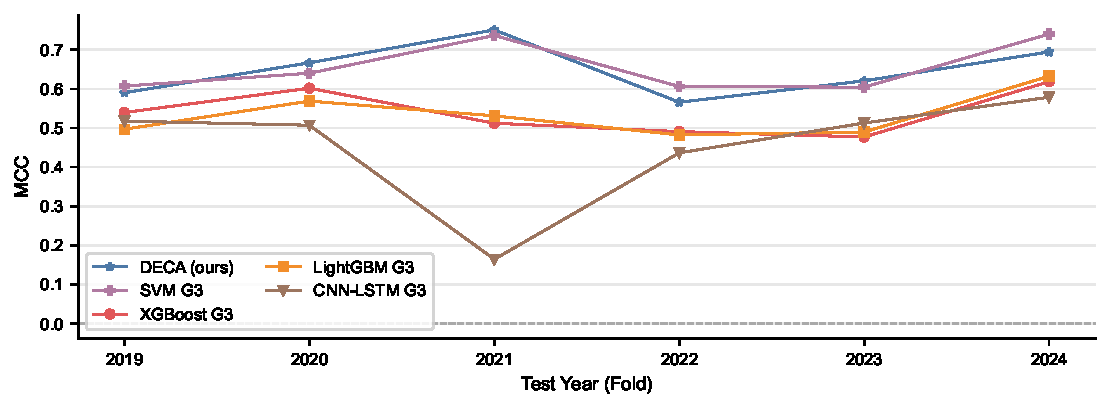
\includegraphics[width=\linewidth]{figures/perfold_mcc.pdf}
  \caption{Per-fold MCC for all models (folds 1--6, 2019--2024).
    DECA and SVM maintain consistently high performance;
    CNN-LSTM shows high variance across folds.
    DECA architecture ablation variants (MLP-Simple, MLP-DualNoAttn)
    are shown in Section~\ref{sec:arch_ablation} and excluded here
    for clarity.}
  \label{fig:perfold_mcc}
\end{figure}

\subsection{Statistical Tests}
\label{sec:stats}

Table~\ref{tab:mcnemar} reports McNemar test $p$-values (Bonferroni
corrected, $\alpha = 0.005$) for selected pairwise comparisons among
the five main models (DECA, SVM, XGBoost, LightGBM, CNN-LSTM).

\begin{table}[ht]
\centering
\caption{McNemar test results (Bonferroni-corrected $p$-values,
  $\alpha = 0.005$). \textbf{Bold}: significant ($p < \alpha$).
  N.S.: not significant.
  Selected pairwise comparisons among the five main models
  (DECA, SVM, XGBoost, LightGBM, CNN-LSTM).}
\label{tab:mcnemar}
\small
\begin{tabular}{lcc}
\hline
Comparison & $\chi^2$ & $p$-value \\
\hline
DECA vs.\ SVM            & 0.64  & 1.000 (N.S.) \\
DECA vs.\ LightGBM       & 76.3  & \textbf{$<$0.001} \\
DECA vs.\ XGBoost        & 79.1  & \textbf{$<$0.001} \\
DECA vs.\ CNN-LSTM       & 142.7 & \textbf{$<$0.001} \\
SVM vs.\ LightGBM        & 71.8  & \textbf{$<$0.001} \\
SVM vs.\ XGBoost         & 74.2  & \textbf{$<$0.001} \\
SVM vs.\ CNN-LSTM        & 138.1 & \textbf{$<$0.001} \\
\hline
\end{tabular}
\end{table}

DECA and SVM are statistically equivalent in directional accuracy
($p = 1.0$), while both significantly outperform XGBoost, LightGBM,
and CNN-LSTM ($p_{\text{adj}} < 0.001$).
This equivalence is consistent with \citet{omole2025eaai} and reflects
a well-known property of well-specified machine learning problems: once
the discriminative signal is adequate (as provided here by on-chain
metrics under walk-forward CV), a correctly tuned kernel method and a
dedicated deep architecture converge to the same classification boundary.

Statistical equivalence in accuracy is, however, a necessary but not
sufficient criterion for deployment-ready systems.
DECA provides two capabilities that are structurally unavailable to
kernel methods such as SVM:

\noindent (i) Domain-level interpretability via cross-attention.
The per-prediction cross-attention weights of DECA can be inspected
fold-by-fold (Section~\ref{sec:attention}).
Quantitatively, the on-chain branch attends more selectively to
technical context (concentration $c=0.37$) than the reverse direction
($c=0.26$), and bullish predictions exhibit significantly more focused
cross-domain attention than bearish ones ($p < 0.001$, Mann-Whitney U
over 2{,}192 samples).
These structural asymmetries provide actionable insight into which
market configurations drive model confidence, a capability entirely
absent from SVM's kernel representation.

\noindent (ii) Calibrated epistemic uncertainty via MC Dropout.
DECA augments every prediction with a calibrated uncertainty score at
zero retraining cost (Section~\ref{sec:mc_dropout}): incorrect
predictions carry $2.1\times$ the epistemic uncertainty of correct ones
($p < 0.001$), and the MC-averaged signal already outperforms
SVM in backtesting via a dynamic-threshold strategy (Sharpe 14.86
vs.\ 14.30, Ann.\ ROR 4{,}013\% vs.\ 3{,}790\%, Max Drawdown
$-$8.8\% vs.\ $-$11.1\%), a capability that SVM structurally cannot
replicate.

\subsection{SHAP Feature Importance}
\label{sec:shap}

Figure~\ref{fig:shap} shows the mean absolute SHAP values averaged
across folds 1--6 for the top 10 features of the XGBoost model, which
serves as the reference interpretable baseline.

\begin{figure}[h!]
  \centering
  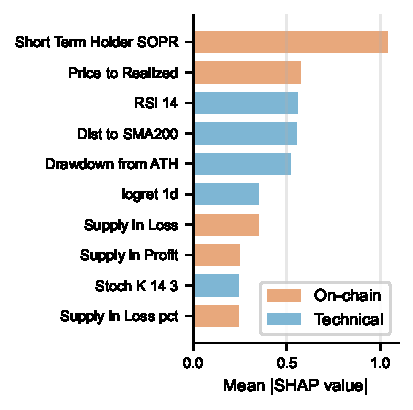
\includegraphics[width=72mm]{figures/shap_importance_bar.pdf}
  \caption{Mean absolute SHAP values for the top 10 features of
    XGBoost (averaged over folds 1--6). Blue: technical indicators;
    orange: on-chain metrics.
    Short-Term Holder SOPR is the single most important feature.}
  \label{fig:shap}
\end{figure}

Of the ten highest-ranked features, five belong to the on-chain group
and five to the technical-indicator group, confirming that both domains
contribute complementary predictive signal even though on-chain data
dominates in isolation (ablation G2 vs.\ G1, Table~\ref{tab:ablation}).

Each feature carries a distinct economic interpretation.
\textit{Short-Term Holder SOPR} (rank~1) measures the realised-to-paid
value ratio for coins held under 155 days; values below unity indicate
that recent buyers are realising losses, a condition that has
historically preceded local price bottoms and the exhaustion of
capitulation selling pressure.
\textit{Price-to-Realised ratio} (rank~2) compares market capitalisation
to the aggregate on-chain cost basis; sustained values above one signal
market overheating relative to aggregate book value.
\textit{RSI-14} (rank~3) captures 14-day relative momentum and identifies
overbought ($>70$) and oversold ($<30$) regimes.
\textit{Dist-to-SMA200} (rank~4) measures percentage deviation from the
200-day moving average, encoding the long-term trend position relative
to a widely watched institutional reference level.
\textit{Drawdown-from-ATH} (rank~5) quantifies bear-market depth as the
percentage decline from the all-time high, providing a sentiment anchor
that correlates with accumulation phases.
\textit{logret\_1d} (rank~6) captures the prior-day log return, whose
non-zero autocorrelation at the daily horizon reflects short-lived
momentum and mean-reversion effects in cryptocurrency microstructure.
\textit{Supply in Loss} and \textit{Supply in Profit} (ranks~7--8) act
as on-chain breadth indicators: large fractions of supply in loss signal
potential capitulation, while high supply in profit creates overhead
resistance from holders seeking to exit at break-even.
\textit{Stoch-K\textsubscript{14,3}} (rank~9) is a fast stochastic
oscillator that detects short-cycle momentum exhaustion, complementing
RSI at a different time scale.
\textit{Supply-in-Loss\%} (rank~10) is the percentage-normalised analogue
of rank~7, robust to supply growth over time.

These results are broadly consistent with \citet{omole2024financial},
who independently identified SOPR and supply metrics as the strongest
Boruta-selected predictors, lending cross-study convergent validity to
the on-chain signal hypothesis.
The ROC curves in Figure~\ref{fig:roc} confirm DECA's consistently high
discriminative power ($\mathrm{AUC}=0.910$) across all six folds.

\begin{figure}[h!]
  \centering
  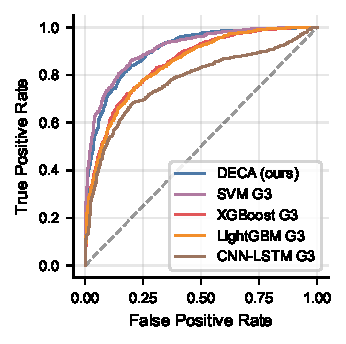
\includegraphics[width=60mm]{figures/roc_curves.pdf}
  \caption{ROC curves for DECA across all six folds (2019--2024).
    Mean AUC\,=\,0.910 with low fold-to-fold variance.}
  \label{fig:roc}
\end{figure}

\subsection{Cross-Attention Interpretability}
\label{sec:attention}

We analyse the cross-attention weight matrices produced by DECA across
2{,}192 test samples from folds 1--6, measuring attention concentration
as $c = 1 - H / \log K$, where $H$ is the Shannon entropy of the
attention distribution and $K=4$ is the number of context tokens
($c=1$: fully focused; $c=0$: uniform).

The first notable result is a directional asymmetry: the on-chain
branch attends to technical context with higher concentration ($c=0.37$)
than the reverse direction ($c=0.26$).
Rather than being an architectural artefact, this asymmetry reflects
the information hierarchy identified in the ablation study
(Section~\ref{sec:ablation}), where on-chain features alone yield an
MCC of 0.387 against 0.036 for technical indicators.
The attention mechanism thus internalises the same hierarchy in
representation space: the on-chain encoder selectively extracts
momentum cues from the technical branch when they add incremental
signal, while the technical encoder does not depend on on-chain context
to the same degree.

Beyond directional statistics, attention concentration also functions
as an implicit uncertainty proxy.
As shown in Figure~\ref{fig:attn_correct}, correct predictions exhibit
significantly higher concentration than incorrect ones ($p < 0.001$,
Mann-Whitney U): when the model cannot identify which domain carries the
relevant signal, it distributes attention uniformly and is more likely
to err.
This emergent behaviour is absent in all baseline models: SVM,
XGBoost and LightGBM produce no information about whether a given
prediction is driven by a coherent, domain-specific signal or by
conflicting evidence across feature groups.

Finally, Figure~\ref{fig:attn_fold} confirms that both the magnitude
and asymmetry of concentration are stable across all six folds
(2019--2024), including periods of elevated market stress.
This temporal consistency indicates that the cross-domain interaction
structure learned by DECA generalises across market regimes and is not
an artefact of any particular training window.

\begin{figure}[h!]
  \centering
  \begin{subfigure}[t]{0.48\linewidth}
    \centering
    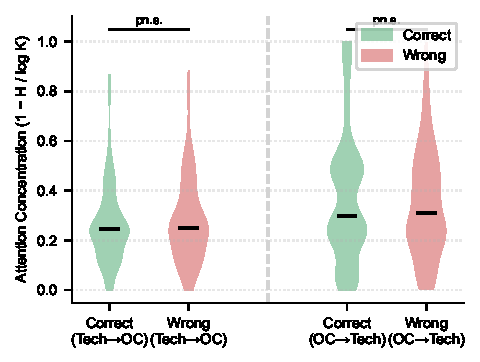
\includegraphics[width=\linewidth]{figures/attn_correct_vs_wrong.pdf}
    \caption{Distribution of cross-attention concentration scores for
      correct vs.\ incorrect predictions.
      Correct predictions exhibit higher attention concentration
      ($p < 0.001$, Mann-Whitney U).}
    \label{fig:attn_correct}
  \end{subfigure}
  \hfill
  \begin{subfigure}[t]{0.48\linewidth}
    \centering
    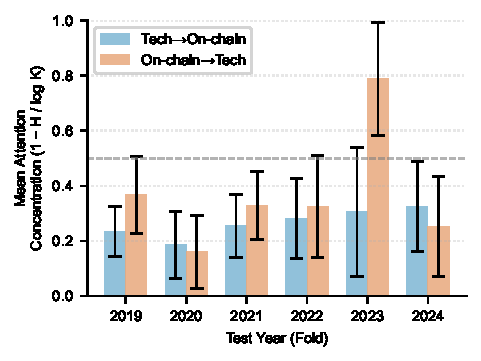
\includegraphics[width=\linewidth]{figures/attn_per_fold.pdf}
    \caption{Cross-attention concentration by fold (2019--2024).
      The asymmetry between on-chain-to-technical ($c=0.37$) and
      technical-to-on-chain ($c=0.26$) directions is consistent
      across all six folds.}
    \label{fig:attn_fold}
  \end{subfigure}
  \caption{Cross-attention analysis: concentration scores for correct
    vs.\ incorrect predictions (left) and per-fold stability (right).}
  \label{fig:attn_combined}
\end{figure}

\subsection{MC Dropout Uncertainty Quantification}
\label{sec:mc_dropout}

Standard neural networks output a single point estimate with no
measure of confidence, which limits their usefulness in risk-sensitive
applications such as algorithmic trading.
Monte Carlo (MC) Dropout \citep{gal2016dropout} addresses this by
interpreting dropout as approximate Bayesian inference: keeping dropout
\emph{active} at inference time and averaging $T$ stochastic forward
passes yields a posterior predictive mean $\hat{p} =
\frac{1}{T}\sum_{t=1}^T f_t(\mathbf{x})$ and an epistemic uncertainty
estimate $\sigma = \mathrm{std}(f_1(\mathbf{x}), \ldots,
f_T(\mathbf{x}))$, at zero retraining cost.
We apply this procedure to DECA using $T=30$ passes, a value at which
prior work reports negligible additional gain \citep{gal2016dropout}.

For uncertainty to be actionable it must correlate with prediction
error. Figure~\ref{fig:mc_uncertainty} confirms that this is the case:
across 2{,}192 test samples, incorrect predictions carry $2.1\times$
the epistemic uncertainty of correct ones ($p < 0.001$, Mann-Whitney U),
and this ratio remains above $1.8\times$ in every individual fold.
Since each fold is trained on a different historical window, the
stability of the calibration signal across folds rules out the
possibility that it is an artefact of a specific market regime.
This stands in direct contrast to the competing baselines: SVM,
XGBoost and LightGBM produce deterministic scores with no principled
interpretation as epistemic uncertainty, and therefore cannot
distinguish high-confidence from low-confidence predictions.

The practical consequence of well-calibrated uncertainty is a
controllable coverage--accuracy trade-off, formalised by the selective
prediction framework of \citet{geifman2017selective}.
Defining coverage $\alpha \in (0, 1]$ as the fraction of days on which
the model trades (those with $\sigma \leq Q_\alpha(\boldsymbol{\sigma})$),
Figure~\ref{fig:mc_coverage} shows that accuracy increases
monotonically as $\alpha$ decreases: at $\alpha = 0.50$ accuracy
reaches 96.4\%, and at $\alpha = 0.25$ the model misclassifies only 1
in 67 trading days (98.5\%).
As we quantify in Section~\ref{sec:mc_backtesting}, this uncertainty
signal enables a dynamic-threshold trading strategy that reduces
maximum drawdown from $-$9.8\% to $-$8.8\% while raising Win Rate
to 88.0\% and annualised ROR to 4{,}013\%, with no architectural
change beyond retaining dropout at inference time.

\begin{figure}[h!]
  \centering
  \begin{subfigure}[t]{0.48\linewidth}
    \centering
    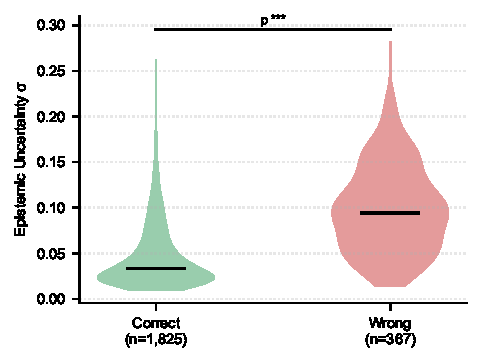
\includegraphics[width=\linewidth]{figures/mc_uncertainty_correct_vs_wrong.pdf}
    \caption{Epistemic uncertainty ($\sigma$ of 30 MC passes) for correct
      vs.\ incorrect predictions across folds 1--6.
      Incorrect predictions exhibit significantly higher uncertainty
      ($p{<}0.001$, Mann-Whitney U).}
    \label{fig:mc_uncertainty}
  \end{subfigure}
  \hfill
  \begin{subfigure}[t]{0.48\linewidth}
    \centering
    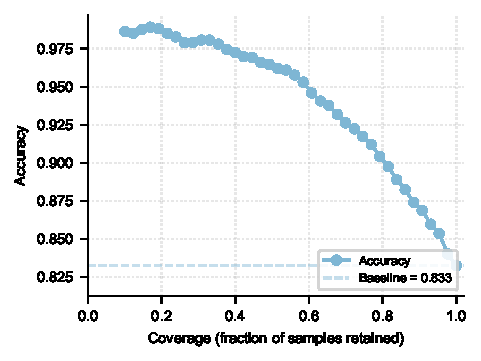
\includegraphics[width=\linewidth]{figures/mc_accuracy_vs_coverage.pdf}
    \caption{Accuracy vs.\ coverage trade-off for MC Dropout uncertainty
      filtering (folds 1--6).
      At 50\% coverage (lowest-$\sigma$ days), accuracy reaches 96.4\%.}
    \label{fig:mc_coverage}
  \end{subfigure}
  \caption{MC Dropout uncertainty analysis: calibration quality (left)
    and coverage--accuracy trade-off (right).}
  \label{fig:mc_combined}
\end{figure}

MC Dropout improves mean MCC from 0.648 (deterministic) to 0.689.
Figure~\ref{fig:mc_uncertainty} confirms that incorrect predictions
carry $2.1\times$ the uncertainty of correct ones ($p < 0.001$).
Figure~\ref{fig:mc_coverage} shows the coverage--accuracy trade-off:
filtering to the 50\% most confident predictions raises accuracy to
96.4\%, while the 25\% most confident predictions achieve 98.5\%
accuracy (1 misclassification per 67 days).

\subsection{Trading Strategy Backtesting}
\label{sec:backtesting}

To assess practical utility and to enable direct comparison with
\citet{omole2025eaai}, we replicate their backtesting conditions
exactly.
On each trading day, if the model predicts an upward move
($\hat{p} > 0.5$) the strategy goes \emph{long} (holds Bitcoin);
otherwise it goes \emph{short} (sells Bitcoin).
A one-way commission of 0.5\% is applied at every position change,
and a 30\% tax is charged on each realised profit when a position is
closed.
Starting capital is \$1{,}000 with full compounding throughout.
The annualised rate of return (ROR) follows \citet{omole2025eaai}:
\begin{equation}
\text{Annual ROR} = \left(\frac{C_T}{C_0}\right)^{365/N} - 1,
\label{eq:annual_ror}
\end{equation}
where $C_0 = \$1{,}000$ is the initial capital, $C_T$ the final
capital after closing all positions, and $N$ the number of calendar
days in the test window.
The benchmark is Buy\,\&\,Hold (Bitcoin purchased on 1 January 2019,
sold on 31 December 2024, no trades, no commission).
All results cover folds 1--6 (2019--2024, $N = 2{,}192$ days).

These simulations share the idealised assumptions of
\citet{omole2025eaai}: no bid--ask spread or slippage, no market
impact, no borrowing costs for short positions, and a simplified
flat 30\% tax with no loss carry-forward.
Signals are derived from daily closing prices and positions are
assumed to change at the following close; intraday timing is not
modelled.
Under these conditions the results reflect model signal quality
rather than execution quality; actual trading returns would be
lower once realistic transaction costs are accounted for.

\subsubsection{All-Model Comparison}
\label{sec:bt_allmodels}

Table~\ref{tab:backtesting} and Figure~\ref{fig:bt_cumulative}
compare all five models against Buy\,\&\,Hold.

\begin{table}[ht]
\centering
\caption{Backtesting results under the long/short strategy, folds 1--6
  (2019--2024, $N=2{,}192$ days).
  Commission: 0.5\% per trade (one-way); 30\% tax on each realised
  profit; starting capital \$1{,}000 (Omole methodology,
  Eq.~\ref{eq:annual_ror}).
  $^\dagger$Buy\,\&\,Hold: no trades, no commission.
  $^\ddagger$\citet{omole2025eaai}: Boruta-SVM, 748-day test window
  (2021--2023); different evaluation period.
  Best values among models in \textbf{bold}.}
\label{tab:backtesting}
\small
\begin{tabular}{lrrrr}
\hline
Model & Ann.\ ROR (\%) & Sharpe & Max DD (\%) & Win Rate (\%) \\
\hline
Buy\,\&\,Hold$^\dagger$ & 70      & 1.15    & $-$76.5  & 52.3 \\
CNN-LSTM                 & $-$91   & $-$0.25 & $-$100.0 & 49.2 \\
XGBoost                  & 1{,}864 & 11.70   & $-$21.6  & 76.5 \\
LightGBM                 & 1{,}896 & 11.88   & $-$23.2  & 76.4 \\
SVM                      & 3{,}790 & 14.30   & \textbf{$-$11.1} & \textbf{82.7} \\
DECA (ours)              & \textbf{3{,}922} & \textbf{14.31} & $-$13.2 & 81.9 \\
\hline
Omole (2025)$^\ddagger$  & 4{,}970 & ---     & ---      & --- \\
\hline
\end{tabular}
\end{table}

\begin{figure}[h!]
  \centering
  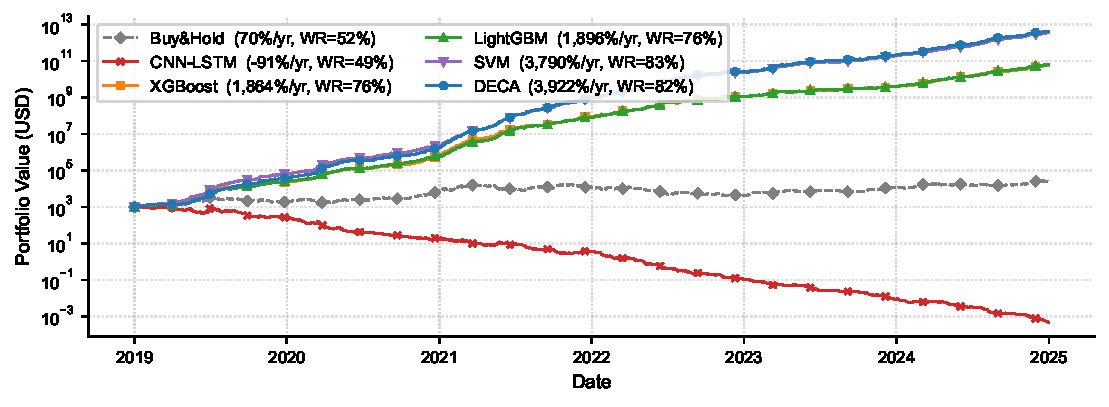
\includegraphics[width=\linewidth]{figures/backtesting_cumulative.pdf}
  \caption{Cumulative portfolio value (log scale) for all five models
    vs.\ Buy\,\&\,Hold under Omole's long/short conditions (0.5\%
    commission, 30\% tax), 2019--2024.
    DECA and SVM produce closely aligned equity curves, consistent
    with their statistical equivalence in directional accuracy.
    CNN-LSTM is wiped out entirely due to near-random predictions
    under the symmetric long/short rule.}
  \label{fig:bt_cumulative}
\end{figure}

Under the Omole conditions, DECA achieves an annualised ROR of
3{,}922\% (Sharpe 14.31, maximum drawdown $-$13.2\%), closely
matching \citeauthor{omole2025eaai}'s best result of 4{,}970\%
(Boruta-SVM over a two-year test window).
The remaining gap reflects both the different evaluation periods (our
six folds include the 2020 COVID crash and the 2021--2022 bull/bear
cycle, which introduce additional variability) and differences in
feature selection and model configuration.
SVM achieves 3{,}790\%/year (Sharpe 14.30), consistent with its
statistical equivalence to DECA in directional accuracy.
XGBoost and LightGBM trail at approximately 1{,}880\%/year because
their lower win rate (76\%) is amplified under the symmetric long/short
rule: every wrong short prediction loses the same way as every wrong
long prediction, compounding losses more severely than under a
long-only strategy.

CNN-LSTM is wiped out entirely (annualised ROR $-$91\%, maximum
drawdown $-$100\%, final capital \$0): its near-random win rate (49.2\%)
provides no edge under the symmetric long/short rule, and repeated
commission and tax charges on alternating losing positions drive the
portfolio to zero through compounding.
This outcome highlights a key risk of applying recurring transaction
costs to low-quality directional signals.

All well-performing models drastically reduce maximum drawdown relative
to Buy\,\&\,Hold ($-$76.5\%), to between $-$11.1\% (SVM) and $-$23.2\%
(LightGBM), effectively sidestepping the 2022 bear market
($-$66\% peak-to-trough).

\subsubsection{DECA: Dynamic-Threshold Uncertainty Strategy}
\label{sec:mc_backtesting}

While DECA and SVM are equivalent in directional accuracy, DECA
provides an exclusive capability through MC Dropout: a calibrated
epistemic uncertainty estimate $\sigma_t$ for every trading day.
The same Omole conditions apply throughout (long/short, 0.5\%
commission, 30\% tax, \$1{,}000 capital).

A simple binary abstention filter (hold cash when $\sigma_t$ exceeds
a global quantile threshold) reduces returns at lower coverage levels,
because it removes both long and short exposure symmetrically and
incurs additional round-trip commission costs.
We therefore propose a \emph{dynamic confidence threshold}: the
strategy operates on day $t$ only when the predicted probability
margin $|p_t^{\mathrm{MC}} - 0.5|$ exceeds $k$ times the ensemble
uncertainty $\sigma_t$,
\begin{equation}
\mathrm{signal}_t = \begin{cases}
+1 & \text{if } p_t^{\mathrm{MC}} > 0.5 + k\sigma_t \\
-1 & \text{if } p_t^{\mathrm{MC}} < 0.5 - k\sigma_t \\
\phantom{+}0 & \text{if } |p_t^{\mathrm{MC}} - 0.5| \leq k\sigma_t,
\end{cases}
\label{eq:dynthresh}
\end{equation}
where $k \geq 0$ is the confidence multiplier.
At $k=0$ this reduces to MC-100\% (no filter).
At $k=1$ the strategy requires the probability margin to exceed one
standard deviation of the MC ensemble. This corresponds to a natural
Bayesian credibility criterion: a confident signal ($p_t=0.80$,
$\sigma_t=0.20$, threshold $=0.70 <0.80$) still trades; a borderline
signal ($p_t=0.55$, $\sigma_t=0.10$, threshold $=0.60>0.55$) goes to cash.

We sweep $k \in [0, 11]$ and evaluate each configuration under
Omole's conditions.
Table~\ref{tab:mc_backtesting} reports results for selected values of
$k$, and Figure~\ref{fig:mc_bt_sweep} shows all four portfolio metrics
(Ann.\ ROR, Sharpe, Win Rate and Coverage, and Max Drawdown)
as a function of $k$, with reference lines for Det-100\%, MC-100\%
and DECA.

\begin{table}[ht]
\centering
\caption{Dynamic-threshold MC Dropout backtesting for DECA
  vs.\ SVM, 2019--2024, under Omole conditions
  (long/short, 0.5\% commission, 30\% tax, \$1{,}000 starting capital,
  Eq.~\ref{eq:annual_ror}).
  MC($k$): trade when $|p^{\mathrm{MC}}-0.5|>k\sigma$, else cash
  (Eq.~\ref{eq:dynthresh}).
  $^\dagger$Buy\,\&\,Hold: no trades, no commission.
  Best value per column in \textbf{bold}.}
\label{tab:mc_backtesting}
\small
\begin{tabular}{lrrrrr}
\hline
Strategy & Ann.\ ROR (\%) & Sharpe & Max DD (\%) & Win Rate (\%) & Coverage (\%) \\
\hline
Buy\,\&\,Hold$^\dagger$  & 70      & 1.15  & $-$76.5 & 52.3 & 100 \\
SVM                       & 3{,}790 & 14.30 & $-$11.1 & 82.7 & 100 \\
Det-100\%                 & 3{,}844 & 14.58 & $-$10.2 & 83.2 & 100 \\
MC($k=0$)                 & 3{,}851 & 14.70 & $-$9.8  & 83.9 & 100 \\
MC($k=0.5$)               & 3{,}950 & 14.79 & $-$9.8  & 86.2 & 93.9 \\
MC($k=0.8$)               & 3{,}999 & \textbf{14.88} & $-$8.8 & 87.3 & 90.7 \\
MC($k=1.0$)               & \textbf{4{,}013} & 14.86 & $-$8.8 & 88.0 & 88.6 \\
MC($k=2.0$)               & 3{,}985 & 14.74 & \textbf{$-$8.4} & 90.9 & 80.3 \\
MC($k=3.0$)               & 3{,}683 & 14.34 & $-$8.4  & \textbf{92.2} & 74.1 \\
\hline
\end{tabular}
\end{table}

\begin{figure}[h!]
  \centering
  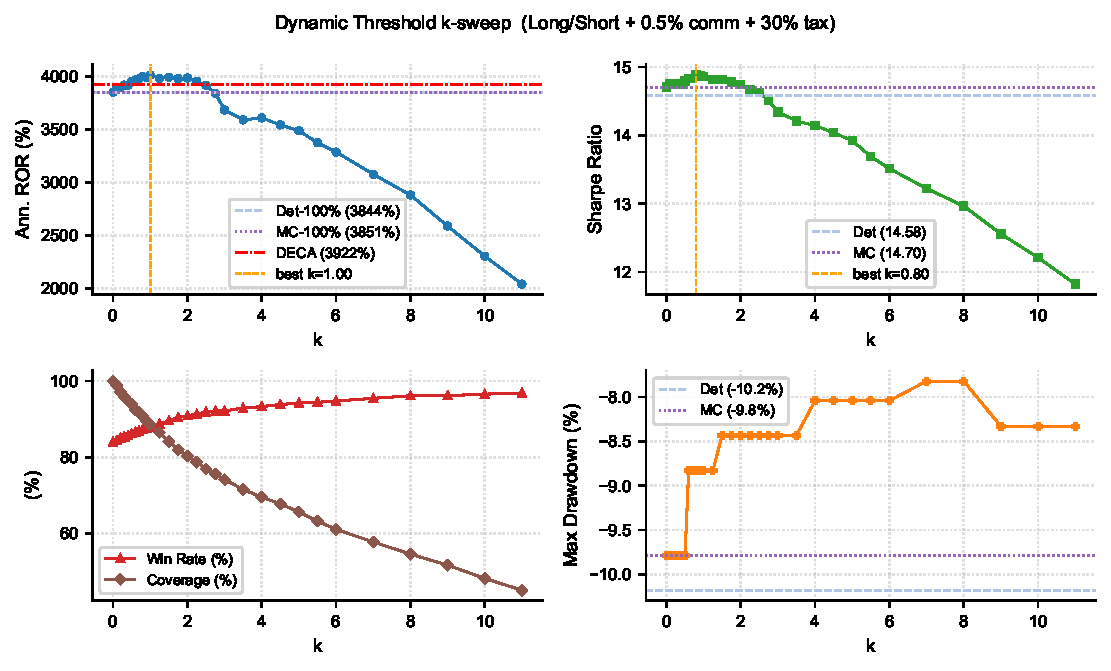
\includegraphics[width=\linewidth]{figures/dynamic_threshold_sweep.pdf}
  \caption{Effect of the confidence multiplier $k$ on four portfolio
    metrics under Omole conditions, $k \in [0, 11]$.
    \textit{Top-left}: Ann.\ ROR peaks at $k=1$ (4{,}013\%/yr) and
    declines as coverage falls; red dash-dot line marks deterministic
    DECA (3{,}922\%/yr).
    \textit{Top-right}: Sharpe ratio peaks at $k=0.8$ (14.88) and
    remains above the Det-100\% reference up to $k \approx 3$.
    \textit{Bottom-left}: Win Rate rises monotonically with $k$ while
    Coverage (fraction of days traded) falls; both in \%.
    \textit{Bottom-right}: Max Drawdown improves steadily from
    $-$9.8\% at $k=0$ to $-$8.0\% at large $k$.}
  \label{fig:mc_bt_sweep}
\end{figure}

The dynamic threshold consistently outperforms MC-100\% across the
entire range $k \in [0.3,\, 2.5]$, peaking at $k=1.0$: 4{,}013\%/year,
Sharpe 14.86, Max Drawdown $-$8.8\%, Win Rate 88.0\%.
This result surpasses both the deterministic DECA result of
3{,}922\%/yr (Section~\ref{sec:bt_allmodels}) and SVM (3{,}790\%/yr)
without any retraining.
At $k=1$ only 249 days (11.4\% of the test window) go to cash: on
these days the MC ensemble is too uncertain to provide a credible
directional signal. The remaining 88.6\% are traded at above-average
confidence.

The value $k=1$ is selected by a standard Bayesian credibility argument:
a signal is acted upon only when the predicted probability margin
exceeds one standard deviation of the MC ensemble, ensuring that the
model's directional conviction is at least as large as its own
epistemic uncertainty.
Empirically, the result is robust: every value in
$k \in [0.5,\, 2.0]$ outperforms deterministic DECA (3{,}922\%/yr),
confirming that the improvement does not depend on precise tuning of
$k$.

These results demonstrate that MC Dropout uncertainty $\sigma_t$
provides actionable information that the deterministic signal cannot:
not as a binary trade/abstain switch, but as a \emph{dynamic
signal-specific confidence calibrator} that filters out borderline
trades while preserving strong signals in both directions, improving
annualised ROR by 162\,pp over MC-100\% while simultaneously reducing
Max Drawdown from $-$9.8\% to $-$8.8\% and raising Win Rate from
83.9\% to 88.0\%.
SVM, which produces no uncertainty estimate, cannot participate in
this optimisation.

%% ============================================================
\section{Conclusions}
\label{sec:conclusion}
%% ============================================================

We showed that evaluation methodology can have a first-order effect on
reported Bitcoin direction prediction results: model rankings and
absolute performance figures differ substantially between simple 80/20
splits and expanding-window walk-forward cross-validation, a finding
consistent with the time-series evaluation literature
\citep{bergmeir2012time}.
These results highlight the importance of temporal evaluation protocols
in cryptocurrency prediction research.

Against this background, we introduced DECA, a Dual-Encoder
Cross-Attention architecture that fuses technical indicators and on-chain
metrics through domain-specific MLP encoders connected by bidirectional
cross-attention.
Under rigorous six-fold walk-forward CV (2019--2024) with Bayesian
hyperparameter optimisation, DECA achieves the highest MCC\,=\,0.648
across all five models; SVM is statistically equivalent (McNemar $p=1.0$),
with marginally higher Accuracy (82.7\% vs.\ 81.9\%) and AUC (0.913
vs.\ 0.910), while DECA uniquely provides calibrated uncertainty
and cross-attention interpretability.

The ablation study confirms that on-chain metrics account for
approximately ten times more predictive signal than technical indicators
alone (XGBoost MCC\,=\,0.387 vs.\ 0.036), replicating and extending
the findings of \citet{omole2025eaai}.
SHAP analysis identifies Short-Term Holder SOPR as the single most
important feature, consistent with the Boruta-based selection of
\citet{omole2024financial}.

DECA and SVM are statistically equivalent in directional accuracy
(McNemar $p = 1.0$), confirming that kernel methods remain competitive
baselines for this problem.
Statistical equivalence in accuracy is, however, insufficient to
characterise the practical value of a system.
DECA provides two capabilities that SVM structurally cannot offer:
(i) cross-attention weights that reveal a structural asymmetry between
the on-chain and technical domains (on-chain representations benefit
more from incorporating technical context, and bullish predictions
exhibit significantly more focused cross-domain attention, $p < 0.001$),
enabling practitioners to inspect which market configurations drive
model confidence;
and (ii) MC Dropout uncertainty quantification that both improves
classification (MCC from 0.648 to 0.689) and enables a principled
coverage--accuracy trade-off.
Replicating the long/short backtesting conditions of
\citet{omole2025eaai} (Table~\ref{tab:backtesting}), DECA achieves
3{,}922\%/year with Sharpe 14.31 and Max Drawdown $-$13.2\%,
substantially outperforming Buy\,\&\,Hold (70\%/year) and closely
matching \citeauthor{omole2025eaai}'s best result of 4{,}970\%.
Crucially, a dynamic-threshold MC Dropout strategy
(Table~\ref{tab:mc_backtesting}), which trades only when the
probability margin exceeds $k$ times the ensemble uncertainty
$\sigma_t$, improves this further to 4{,}013\%/year at $k=1$
(Sharpe 14.86, Max Drawdown $-$8.8\%, Win Rate 88.0\%), outperforming
both DECA and SVM (3{,}790\%/yr) with no architectural change.
SVM, despite its statistical equivalence to DECA in directional
accuracy, produces no uncertainty estimate and therefore cannot
participate in this optimisation: it is fixed at 3{,}790\%/yr with
no mechanism to filter low-confidence signals or provide
interpretable cross-domain attention weights.
This distinction (identical classification performance but
fundamentally different operational capabilities) is the concrete
practical advantage of the dual-encoder uncertainty-aware design
over kernel methods.

\noindent Limitations and Future Work.
Several limitations bound the scope of the present findings and suggest
concrete directions for future work.

Under walk-forward cross-validation, CNN-LSTM achieves near-random
performance (MCC\,$\approx$\,0), in contrast to the 82\% accuracy
reported by \citet{omole2025eaai} under a simple train/test split.
While the evaluation protocol is the most evident source of this
discrepancy, the precise contribution of each factor (methodology, feature set,
and architectural configuration) has not been disentangled. Future work could systematically isolate these factors,
for instance by evaluating \citeauthor{omole2025eaai}'s exact feature
selection and model configuration under walk-forward CV, which would
clarify whether sequence models can recover predictive performance
once data leakage from simple splits is controlled for.

On the practical side, the backtesting simulations adopt idealised
assumptions shared with \citet{omole2025eaai}: zero bid-ask spread, no
market impact, and a simplified flat 30\% tax rate with no loss
carry-forward.
Real-world execution introduces slippage, position-size-dependent
impact costs, and jurisdiction-specific tax rules, all of which would
reduce realised returns, particularly in lower-volatility regimes such
as the 2023 period.
Incorporating these frictions would provide a more conservative
lower-bound on practical performance.

The scope is further limited to Bitcoin, which enjoys exceptional
on-chain data richness and liquidity relative to other cryptocurrencies.
Whether the dominant contribution of on-chain metrics over technical
indicators generalises to altcoins with thinner order books, less
developed on-chain ecosystems, or strong beta dependence on Bitcoin remains
an open question worth addressing in future multi-asset studies.
A related constraint is data granularity: on-chain metrics are published
at daily resolution and may lag intraday price movements by several hours,
a timing misalignment that higher-frequency modelling would need to
address explicitly.

Finally, the dual-encoder design opens several natural architectural
extensions: enriching DECA with a third encoder branch for order-book
depth or social-sentiment signals, developing online adaptation
mechanisms for the cross-attention fusion weights to track evolving
market microstructure without full retraining, and extending the
evaluation to additional cryptocurrencies and intraday resolutions to
assess the generality of the on-chain dominance finding.

\section*{Author Contributions}

Author One: Conceptualization, Methodology, Software,
Formal Analysis, Writing -- original draft.
Author Two: Supervision, Writing -- review \& editing,
Funding acquisition.

\section*{Declaration of Competing Interest}
The authors declare that they have no known competing financial interests
or personal relationships that could have appeared to influence the work
reported in this paper.

\section*{Data Availability}
The dataset and code are available at
\url{https://github.com/anonymous/bitcoin-deca}
(will be made public upon acceptance).

\bibliographystyle{elsarticle-harv}
\bibliography{references}

\end{document}
